%!TEX root = ../../main.tex
\section{Processing aperture measurements}
\label{sec:Processing aperture measurements}
Prior to the measurements reported here (July 2013), users at Diamond Light Source (DLS) beamline I02 were provided with the full width half maximum (FWHM) values of the X-ray beam measured by a 10$\,\mu m$ aperture (see below).
To obtain a more realistic value of the FHWM it was recommended that 5$\,\mu m$ be subtracted from the supplied FWHM values.
This recommendation however was not supported by any systematic experiments or studies.

For this reason investigations were carried out to obtain a better estimate of the true beam profile to so that a more trustworthy value of the FWHM could be provided to users.
This was the initial motivation for processing beam measurements made using aperture scans.

\subsection{Experimental methods}
\label{sub:Experimental Methods - DLS}
Aperture scans to obtain X-ray beam flux measurements were carried out in collaboration with Dr. Carina Lobley on the DLS I02 beamline.
For these scans, a miniap device, a piece of steel with a 10$\,\mu m$ diameter circular hole, is translated across the beam by remote control.
The position of the aperture is recorded along with a measure of the current detected in a silicon diode (S3590-09 model purchased from Hamamatsu) on the detector shutter (i\_pin) \cite{owen2009}.
The detector current is proportional to the beam flux (photons/second).
First the `centre' $x$ and $y$ position is found such that the diode reading at this position gives the highest current.
The aperture is then translated 120$\,\mu m$ in the negative horizontal direction.
Measurements of the $x$ and $y$ positions and the diode reading are carried out at 2$\,\mu m$ intervals as the aperture is translated across in the positive horizontal direction for a total of 240$\,\mu m$ (+120$\,\mu m$ from the centre).
A similar scan is then carried out in the vertical direction.
Examples of data from the measurements are shown in Figure \ref{fig:Original aperture measurments - DLS}.
\begin{figure}
        \centering
        \begin{subfigure}[b]{1.0\textwidth}
                \centering
                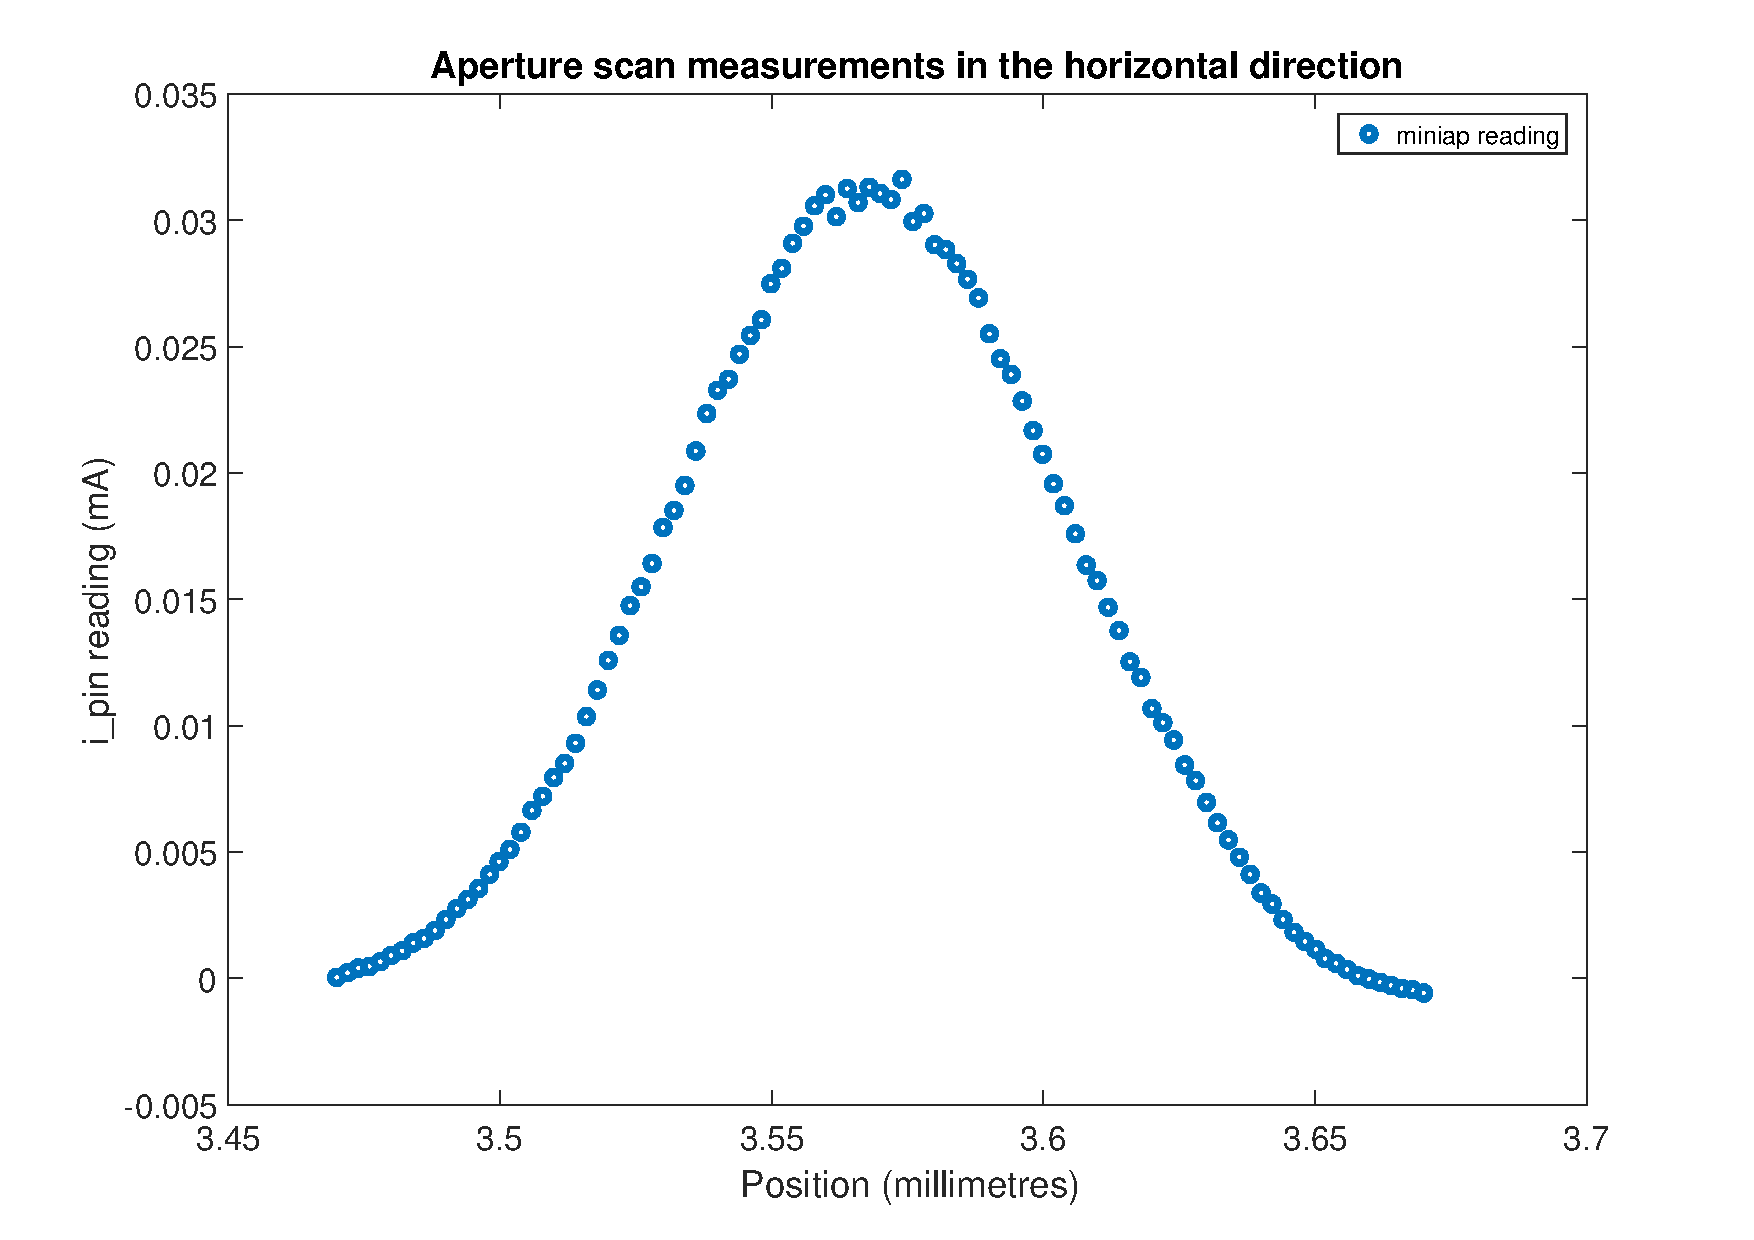
\includegraphics[width=\textwidth]{figures/beam/ApertureScans_x_data.pdf}
                \caption{}
                \label{fig:Original aperture measurments inx-direction - DLS}
        \end{subfigure}
				\\
        \begin{subfigure}[b]{1.0\textwidth}
                \centering
                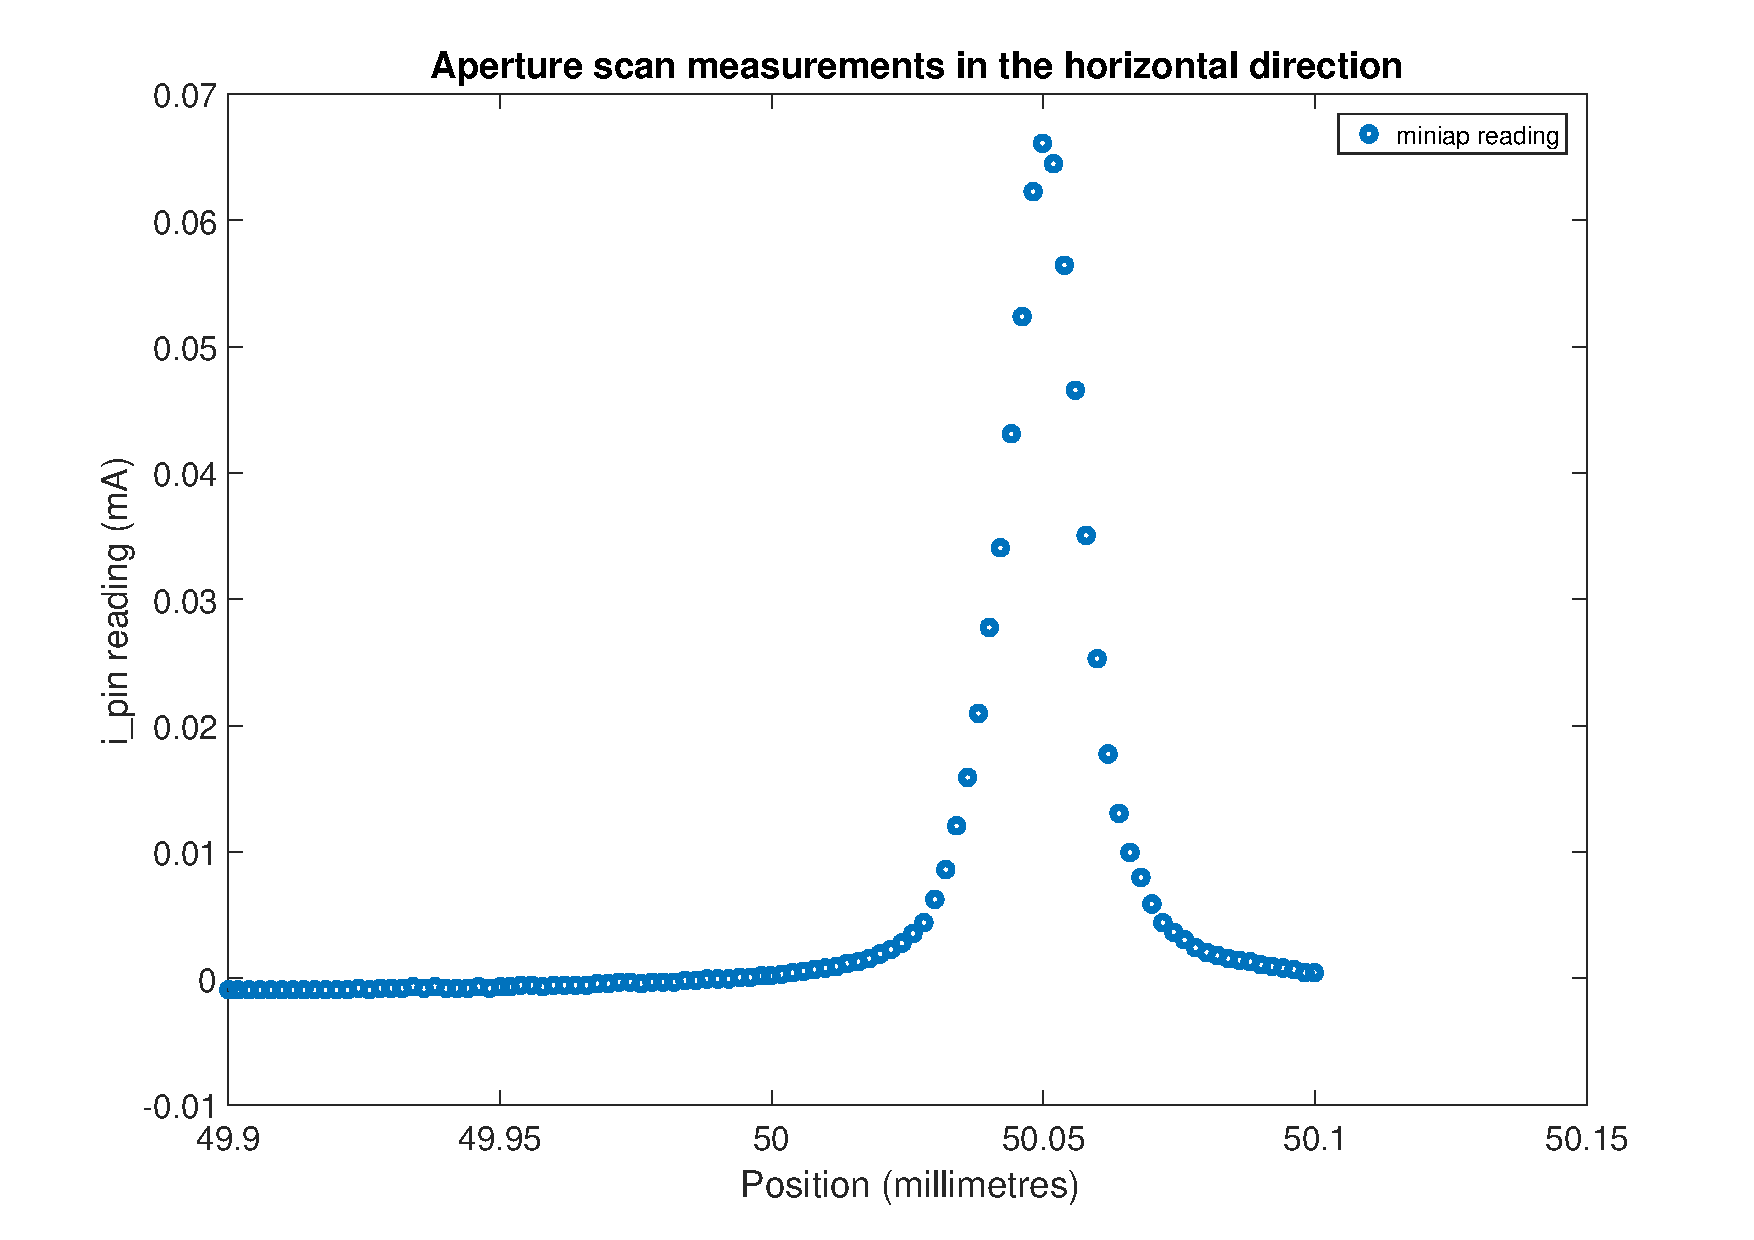
\includegraphics[width=\textwidth]{figures/beam/ApertureScans_y_data.pdf}
                \caption{}
                \label{fig:Original aperture measurments in y-direction - DLS}
        \end{subfigure}
        \caption[Flux measurements collected using 1D aperture scans at the Diamond Light Source synchrotron.]{Examples of the flux measurement data collected at the Diamond Light Source synchrotron.
        The horizontal axis represents the aperture position in millimetres and the vertical axis represents the current in the diode (mA).
        (a) Data collected in the $x$-direction.
        (b) Data collected in the $y$-direction.}
        \label{fig:Original aperture measurments - DLS}
\end{figure}

\subsection{Deconvoluting the X-ray beam measurements}
\label{sub:Deconvolving the X-ray beam measurements}

\subsubsection{Theoretical introduction}
\label{subs:Theoretical introduction}
The area of the aperture used on I02 is (10/2)$^2 \times \pi \approx$ 78.54$\,\mu m^2$, so each diode reading at a position ($x, y$) is the result of the integral of the flux from a 78.54$\,\mu m^2$ area surrounding the central point (Figure~\ref{fig:Aperture scan model - DLS}).
Given that the diode measurements were taken at 2$\,\mu m$ intervals, it is possible to deconvolute the measured signal to obtain a truer value of the diode current to a spatial resolution of 2$\,\mu m$.
Only this estimate of the true 2D profile of the current is necessary for the beam profile measurement. This is because RADDOSE-3D additionally requires a total flux estimate, which is distributed across the measured beam profile (a 2D array) according to the current at each spatial position.
\begin{figure}
    \centering
    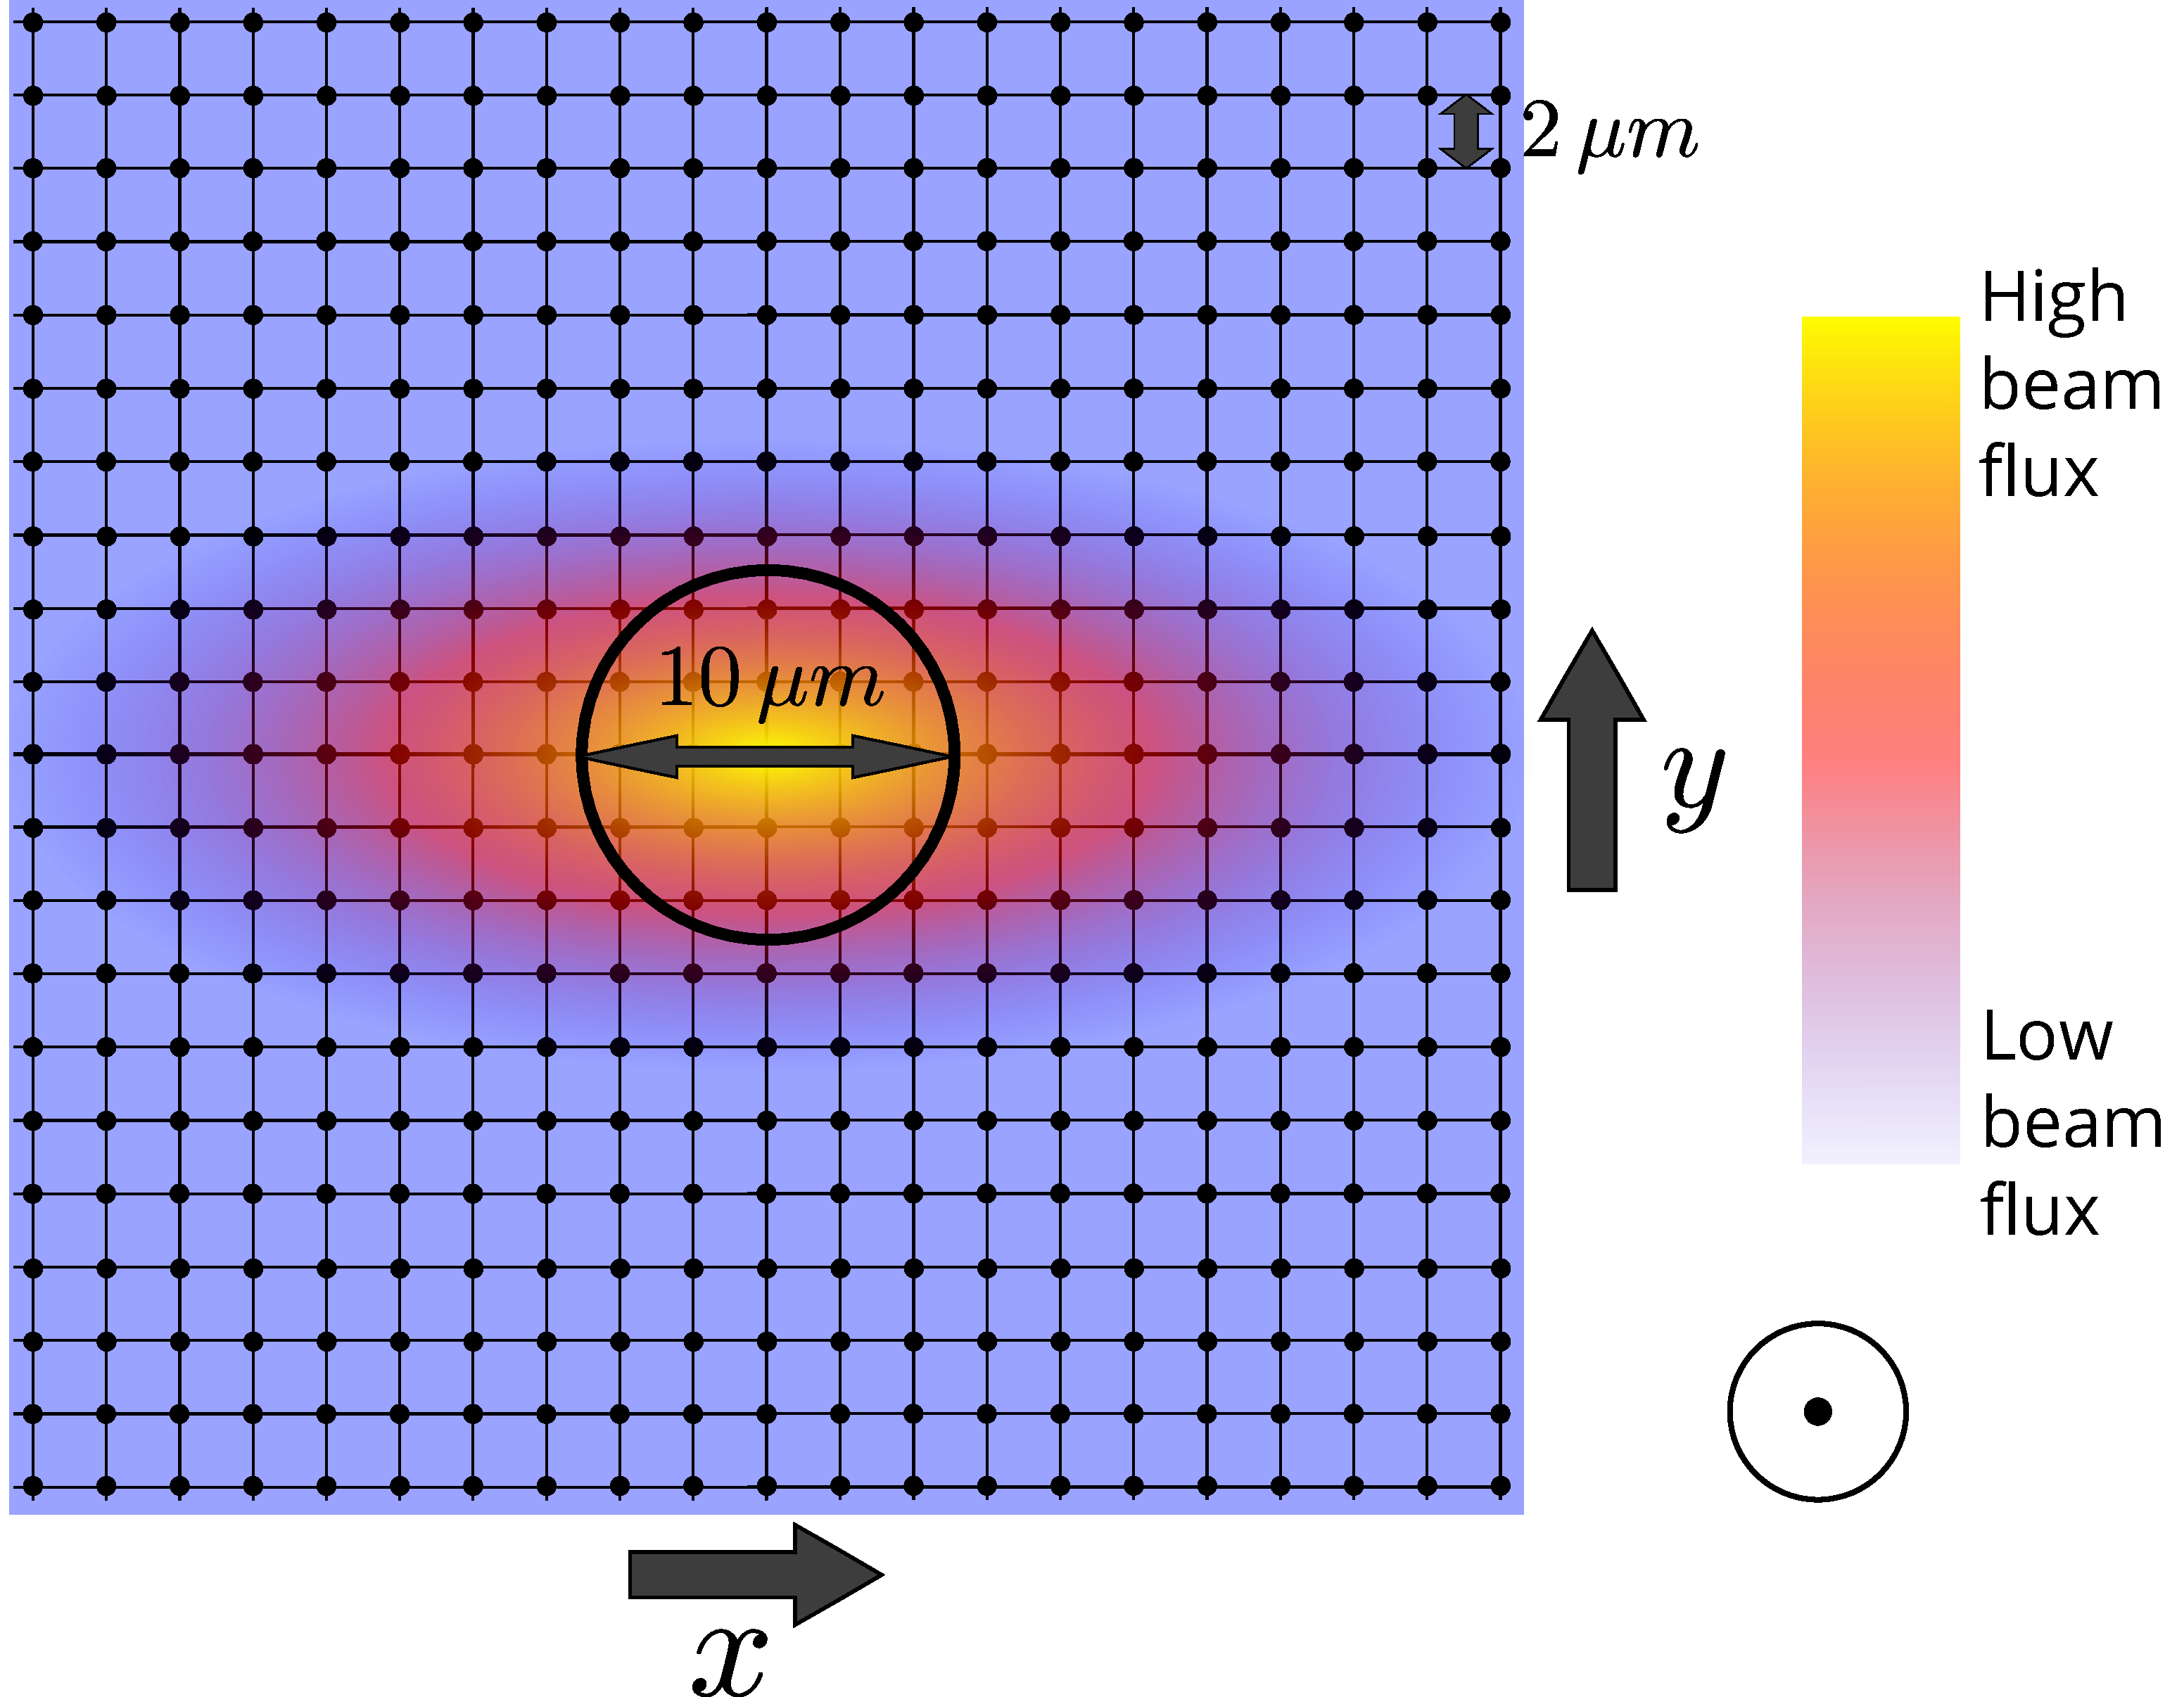
\includegraphics[width=1\textwidth]{figures/beam/aperture_scan_drawing.pdf}
    \caption[A schematic of the X-ray beam and aperture setup.]{A schematic of the X-ray beam and aperture setup as viewed from the detector looking into the beam.
    Each point represents a spatial position where a beam measurement is taken, hence the distance between any two horizontally or vertically consecutive spots is 2$\,\mu m$.
    The circle represents the circular aperture which has a 10$\,\mu m$ diameter.
    The colour represents the beam flux intensity (not to scale).
    The beam is smaller in the $y$ direction than it is in the $x$ direction.
    This diagram shows that a reading at a particular point in space is the integral of all surrounding points within the aperture area.
    Thus the reading of the total X-ray beam profile that is measured is a convolution of readings from local surrounding space.}
    \label{fig:Aperture scan model - DLS}
\end{figure}

To define the problem mathematically, the diode readings can be described as a convolution of the true diode current, $f$, at a point $\bs{x}$, and the area of the aperture, $g$.
Explicitly this is
\begin{equation}
[f*g](\bs{x}) = \int_0^{\bs{x}} f(\bs{u})g(\bs{x}-\bs{u})\mathrm{d}\bs{u} + n(\bs{x}),
\label{eq:Convolution equation with noise}
\end{equation}
where $[f*g]$ is the measured diode reading and $n(\bs{x})$ represents the additive noise at a particular point in space.
The aim of deconvolution in this context is to find the diode current profile, $f(\bs{x})$, given knowledge of the measured current, $[f*g](\bs{x})$, and the aperture contribution, $g(\bs{x})$.
Mathematically this aim can be interpreted as finding some $w(x)$ such that:
\begin{equation}
    \hat{f}(x) = [w * [f*g]](x),
    \label{eq:Wiener aim}
\end{equation}
where $\hat{f}(x)$ is an estimate of $f(x)$ that minimises the mean square error.
In general, deconvolution is an ill-posed problem, thus it is likely that a unique solution does not exist \cite{wolfram2016Deconvolution}.
If it is assumed that the noise has zero mean and is spatially independent (white noise assumption) then the Wiener filter \cite{wiener1949extrapolation} can be used to deconvolute the signal to find $f$.
The Wiener Filter, $W$, is defined mathematically in the Fourier domain as:
\begin{equation}
W = \f{1}{\mathscr{F}(g)}\left[\f{|\mathscr{F}(g)|^2}{|\mathscr{F}(g)|^2 + \f{\mathscr{F}(n)}{\mathscr{F}(f)}}\right],
\label{eq:Wiener Filter}
\end{equation}
where $\mathscr{F}$ denotes the Fourier transform of its argument:
\begin{equation}
\mathscr{F}[f(x)](k) = \int_{-\infty}^{\infty} \! f(x) e^{ikx} \mathrm{d}x.
\label{eq:Classic Fourier Transform}
\end{equation}
The $\f{\mathscr{F}(n)}{\mathscr{F}(f)}$ term in equation \ref{eq:Wiener Filter} is similar to the inverse of a signal to noise ratio in the Fourier domain.
If this value is known exactly, then the Wiener filter often works very well.
However, more commonly the value of this ratio is unknown, and it is often treated as a constant value throughout the domain.
\newline
The Wiener filter is multiplied with the convoluted function in the Fourier domain to give
\begin{equation}
\mathscr{F}[\widehat{f}] = W \mathscr{F}[f*g],
\label{eqwienapp}
\end{equation}
such that $\mathscr{F}[\widehat{f}]$ is the solution found with the minimum mean squared error:
\begin{equation}
\text{error} = E\left[ \left(\mathscr{F}[f]-\mathscr{F}[\widehat{f}]\right)^2\right],
\label{eqerr}
\end{equation}
where the true solution is denoted $\mathscr{F}[f]$.
Multiplication in the Fourier domain is equivalent to a convolution operation in the real domain, making clear the equivalence between equation \ref{eqwienapp} and the statement of the mathematical aim (equation \ref{eq:Wiener aim}).
Parseval's theorem implies that minimising the mean squared error in the Fourier domain is equivalent to minimising the mean squared error in the real domain. For further details on the Wiener Filter and its formal derivation the reader is referred to Gonz\'{a}lez and Woods (1992) \nocite{gon1992}.

\subsubsection{Implementing the deconvolution}
\label{subs:Implementing the deconvolution}
The deconvolution algorithm was implemented in Matlab R2012a.
First the initial diode measurements were read into Matlab and a one-dimensional Gaussian function was fitted to the data in order to obtain the parameter values in both the $x$ and $y$ directions (Figure \ref{figgfit}).
\begin{figure}
        \centering
        \begin{subfigure}[b]{1.0\textwidth}
                \centering
                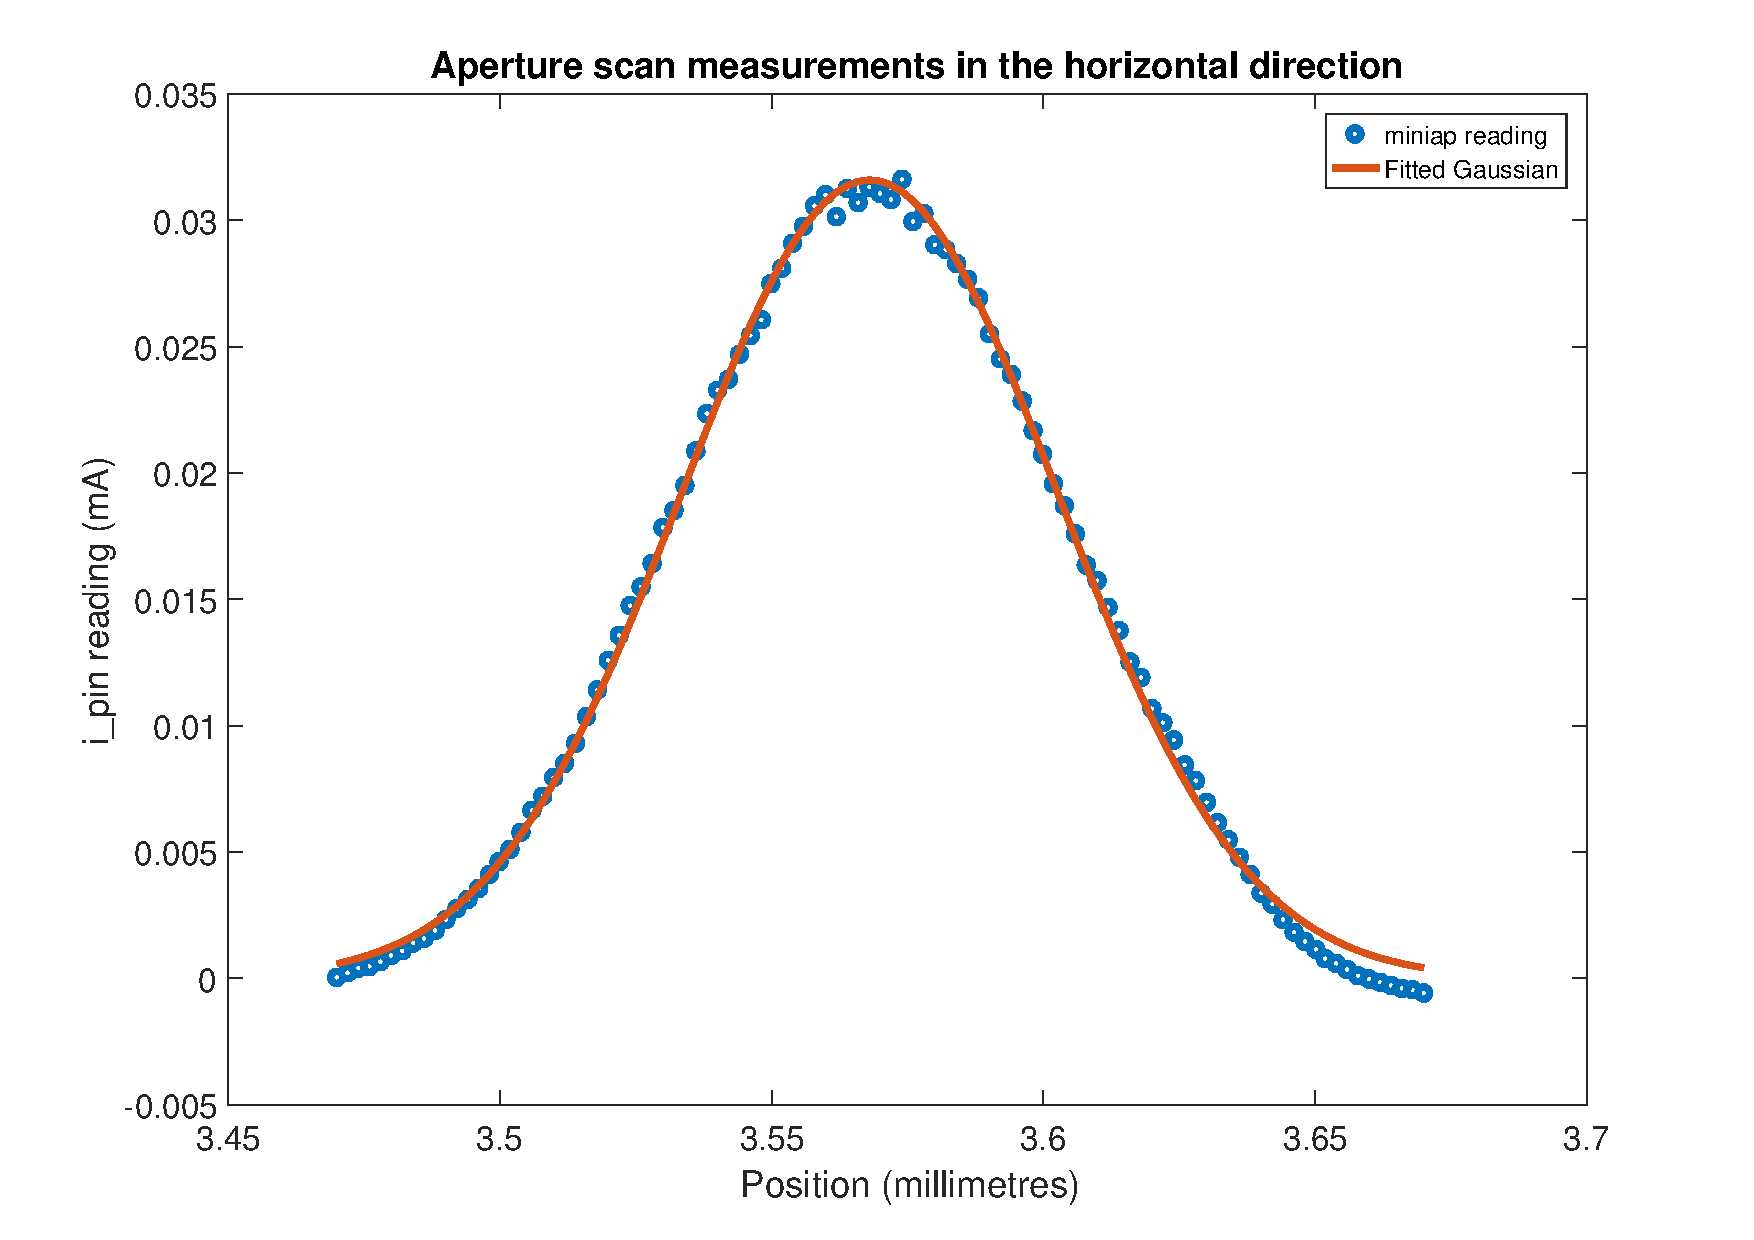
\includegraphics[width=\textwidth]{figures/beam/ApertureScans_x.pdf}
                \caption{}
                \label{figfitx}
        \end{subfigure}
				\\
        \begin{subfigure}[b]{1.0\textwidth}
                \centering
                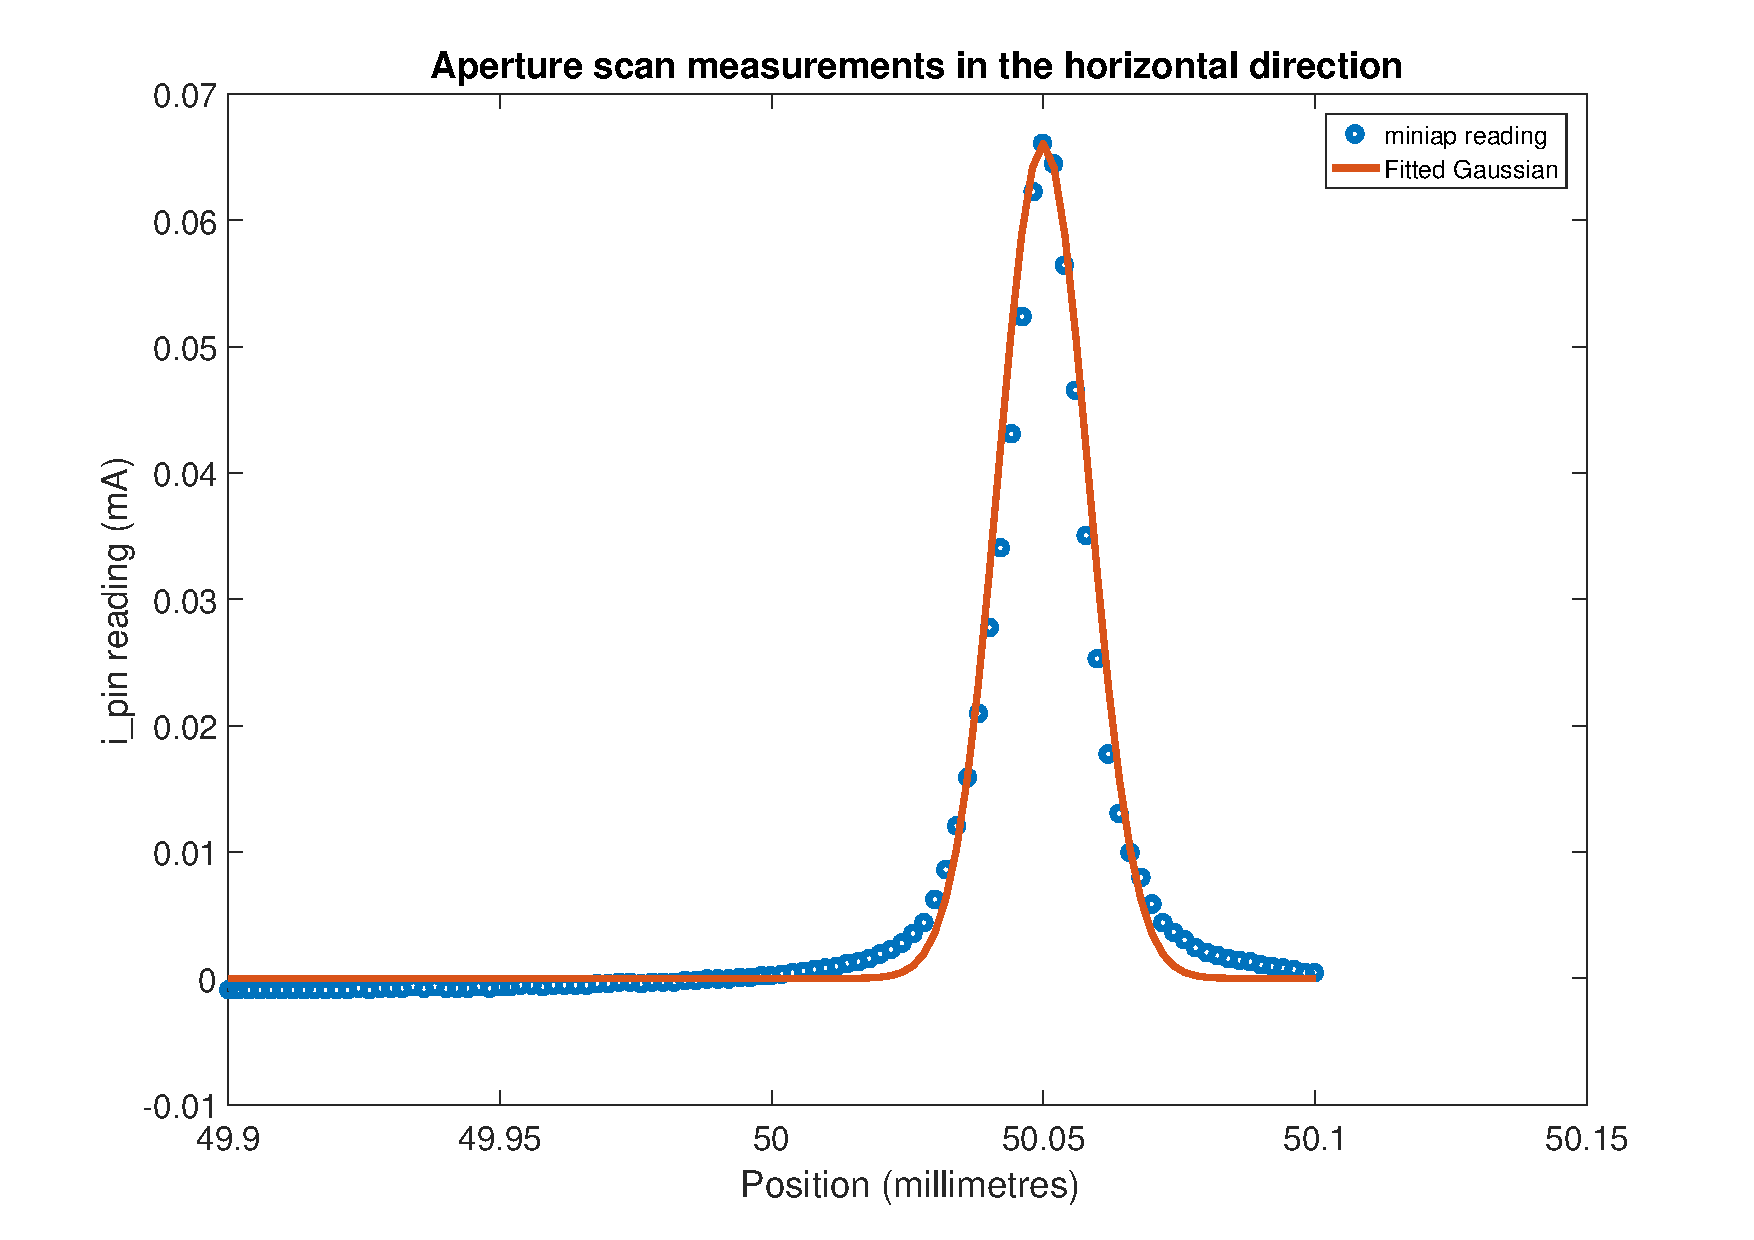
\includegraphics[width=\textwidth]{figures/beam/ApertureScans_y.pdf}
                \caption{}
                \label{figfity}
        \end{subfigure}
        \caption[Aperture scan measurements and the Gaussian fits to the data.]{The original miniap readings from translating the 10$\,\mu m$ diameter aperture are shown as blue circles and the solid orange line is the Gaussian fit to the data.
        (a) beam profile in the $x$-direction.
        (b) beam profile in the $y$-direction.
        Data collected on I02, DLS.}
        \label{figgfit}
\end{figure}
The parameter values were subsequently used for the two-dimensional Gaussian function representing the estimate of the convoluted two dimensional beam profile (Figure~\ref{fig:Gaussian approximation of convolved Beam profile - DLS}).
\begin{equation}
g_{2D}(x,y) = A_{max}\exp\left[-\left(\f{(x - \mu_x)^2}{2\sigma_x^2} + \f{(y - \mu_y)^2}{2\sigma_y^2}\right)\right],
\label{eq:2D Gaussian Function - DLS}
\end{equation}
where $\mu_x$, $\mu_y$, $\sigma_x$ and $\sigma_y$ are the parameters whose values are obtained from fitting the one-dimensional Gaussian functions
\begin{align}
g_h(x) &= A_{x}\exp\left[-\f{(x - \mu_x)^2}{2\sigma_x^2}\right], \label{eq:1D Guassian Function x} \\
g_v(y) &= A_{y}\exp\left[-\f{(y - \mu_y)^2}{2\sigma_y^2}\right], \label{eq:1D Guassian Function y}
\end{align}
and $A_{max}$ is the maximum value of $A_{x}$ and $A_{y}$ which are the values of the highest recorded diode current in the $x$ and $y$ directions respectively.
If the measurements are taken perfectly (i.e. aperture is scanned exactly across the maximum flux in $x$ and $y$) then $A_{x} = A_{y}$, but due to experimental error this is rarely the case.
\newline
To obtain an estimate of the true relative X-ray beam profile, equation \ref{eq:2D Gaussian Function - DLS} has to be deconvoluted with a matrix that corresponds to the aperture.
The aperture matrix is a square matrix created just large enough to contain the area of the circular aperture.
It essentially acts as a mask, so elements of the matrix contain the value 1 if the area is inside the aperture, and 0 if the element is outside the aperture.
To determine the position of a matrix element with respect to the aperture area, each point in the matrix is given the value of the Euclidean distance away from the central matrix element.
This central element is assumed to be at the position of the centre of the aperture.
Any points with a Euclidean distance smaller than the aperture radius are determined to lie within the aperture area and hence given a value of 1.
However points with a Euclidean distance bigger than the aperture radius are outside and are set to 0.
\newline
The $\f{\mathscr{F}(n)}{\mathscr{F}(f)}$ term in equation \ref{eq:Wiener Filter} is estimated using the \verb+fminsearch+ minimisation function in Matlab.
Thus an objective function was written as follows:
\begin{enumerate}
    \item first an estimate of the signal to noise ratio is passed to the objective function
    \item using the estimates a deconvolution of the signal is performed using the two-dimensional beam profile given by equation \ref{eq:2D Gaussian Function - DLS} and the aperture matrix.
    \item a convolution of the deconvoluted signal with the same aperture matrix is performed.
    \item the Frobenius norm\footnote{The Frobenius norm, $||A||_F$, of a matrix, $A$, is defined as $||A||_F \equiv \sqrt{\sum_{i=1}^{m} \sum_{j=1}^{n} |a_{ij}|^2}$ where the $a_{ij}$ represent the elements of the matrix.} of the original convoluted signal subtracted from the newly calculated convoluted signal is calculated and returned by the objective function.
\end{enumerate}
If the two signals give a norm value of zero then they are exactly the same, but otherwise a positive value is returned.
The \verb+fminsearch+ function returns the value of $\f{\mathscr{F}(n)}{\mathscr{F}(f)}$ that minimises the objective function.
Given the convoluted two-dimensional beam profile, the aperture matrix and $\f{\mathscr{F}(n)}{\mathscr{F}(f)}$, the beam profile can be deconvoluted using the Matlab function \verb+deconvwnr+ which performs a Wiener deconvolution as described in section \ref{subs:Theoretical introduction} (Figure~\ref{fig:Deconvolved 2D beam profile - DLS} ).
\begin{figure}
        \centering
        \begin{subfigure}[b]{1.0\textwidth}
                \centering
                \includegraphics[width=\textwidth]{figures/beam/convolved_2d_beam.pdf}
                \caption{}
                \label{fig:Gaussian approximation of convolved Beam profile - DLS}
        \end{subfigure}
				\\
        \begin{subfigure}[b]{1.0\textwidth}
                \centering
                \includegraphics[width=\textwidth]{figures/beam/deconvolved_2d_beam.pdf}
                \caption{}
                \label{fig:Deconvolved 2D beam profile - DLS}
        \end{subfigure}
        \caption[2D X-ray beam profile reconstructions.]{2D X-ray beam profiles.
        (a) Gaussian approximation of the measured current profile given by equation \ref{eq:2D Gaussian Function - DLS}
        (b) Beam profile after Wiener deconvolution.}
        \label{fig:2D relative X-ray beam profiles, convolved and deconvolved}
\end{figure}

The deconvoluted 2D beam profile is not smooth, which is typical of deconvolution when the exact noise distribution is unknown.
A further 2D Gaussian function is fitted to the deconvoluted data in order to obtain a smooth beam profile (Figure~\ref{fig:Gaussian model fitted to the 2D deconvolved profile - DLS}).
This is carried out by taking 1D slices of the 2D beam profile in both the $x$ and the $y$ directions around the slice that gives the maximum readings in the centre, and then obtaining the parameters as outlined above (section \ref{subs:Implementing the deconvolution}).
\begin{figure}
    \centering
    \includegraphics[width=1\textwidth]{figures/beam/gaussian_fitted_deconvolved_2d_beam.pdf}
    \caption[Gaussian model fitted to the deconvoluted X-ray beam profile.]{Gaussian model fitted to the deconvoluted X-ray beam profile (Figure~\ref{fig:Deconvolved 2D beam profile - DLS}).}
    \label{fig:Gaussian model fitted to the 2D deconvolved profile - DLS}
\end{figure}

Using the fitted Gaussian model, any properties of the beam can be determined, such as the Full Width at Half Maximum (FWHM) of the beam, which can then be provided to the I02 DLS users.
The FWHM is defined mathematically for a Gaussian as
\begin{equation}
FWHM = 2 \sigma \sqrt{2\ln(2)}.
\label{eq:FWHM mathematical definition}
\end{equation}

\subsubsection{Validation of deconvolution approach}
\label{subs:Validation of deconvolution approach}
No measuring device is available to take measurements at the resolution to which the deconvolution method attempts to spatially resolve the flux readings.
Therefore to validate the results, the deconvolution method was used in reverse to predict the FWHM values that would be obtained from the diode readings with a 20$\,\mu m$ diameter aperture.
To achieve this the 2D deconvoluted signal (Figure~\ref{fig:Gaussian model fitted to the 2D deconvolved profile - DLS}) was convoluted with an aperture matrix of a different size.
1D slices in the $x$ and $y$ directions were then found such that the flux in the central matrix element was maximum and 1D Gaussian functions were fitted to each slice.
FWHM values were then calculated from the 1D Gaussians using equation \ref{eq:FWHM mathematical definition} and these calculated values could then be compared with the readings taken from actual experimental data obtained using a 20$\,\mu m$ aperture.

\subsection{Results}
\label{sub:Results - DLS}
FWHM values obtained from the experimentally measured (convoluted) i\_pin readings using the 20$\,\mu m$ diameter aperture (referred to as Exp$_{\text{20}}$) were compared with calculated FWHM values derived from the numerical convolution of the deconvoluted profile with the 20$\,\mu m$ aperture (referred to as Conv$_{\text{20}}$ - Table~\ref{tab:FWHM comparison - DLS}).
\begin{table}[h!]
	\caption[Comparison of calculated FWHM values with experimentally observed FWHM values.]{Comparison of calculated FWHM values with experimentally observed FWHM values.
    The calculated FWHM values using the 10$\,\mu m$ aperture (in italics) are calculated from the deconvoluted profile.
    Thus they were not expected to match the experimental values.}
	\begin{tabular}{p{2.5cm} p{2.5cm} p{2cm} p{1.5cm} p{2cm} p{1.5cm}}
        &  Aperture diameter ($\mu m$) & FWHM in $x$ ($\mu m$) 	&	\% Error in $x$		& FWHM in $y$ ($\mu m$) 	&	\% Error in $y$ \\
		\hline
		Exp$_{\text{10}}$         & 10              & 81.6 	            &	0.49      & 19.5 	        & 4.84	\\
		Deconv$_{\text{10}}$      & \textit{10}     & \textit{81.2}     &  	          & \textit{18.6} 	&		\\
                                  &                 &			        &			  &    		        &		\\
        Exp$_{\text{20}}$         & 20              & 81.8              &   2.57      & 21.9            & 1.83  \\
		Conv$_{\text{20}}$        & 20              & 83.9              &             & 22.3            &    	\\
	\end{tabular}
	\label{tab:FWHM comparison - DLS}
\end{table}
The calculated FWHM for Conv$_{\text{20}}$ are quite accurate, showing less than a 3\% error in both the $x$ and $y$ directions when compared to Exp$_{\text{20}}$.
This suggests that the deconvolution method used provides reasonable estimates of the 2D X-ray beam profile.

FWHM values obtained from the experimentally measured (convoluted) i\_pin readings using the 10$\,\mu m$ diameter aperture (referred to as Exp$_{\text{10}}$) were compared with calculated FWHM values derived from the deconvoluted profile with the 10$\,\mu m$ aperture (referred to as Deconv$_{\text{10}}$ - Table~\ref{tab:FWHM comparison - DLS}).
The errors of the FWHM values between Exp$_{\text{10}}$ and Deconv$_{\text{10}}$ are also quite small.
In theory however, these values do not necessarily have to be close because the FWHM from Deconv$_{\text{10}}$ are calculated from the deconvoluted profile, whereas the FWHM from Exp$_{\text{10}}$  are calculated from the convoluted beam profile.
The fact that these values are close provide evidence that users should not subtract 5 $\mu m$ from the quoted FWHM values.
Furthermore it indicates that deconvoluting the X-ray beam does not significantly change the X-ray beam profile.
This is important because it suggests that the measured 2D current profile does not have to be further altered once the profile has been generated from the 1D aperture scans.
